% ---------------------------- Preamble starts here ----------------------------

\documentclass[aspectratio=169]{beamer} %Remove [aspectratio=169] to get non-wide 4:3 slide aspect ratio

%-----------------------------------------------
% --- Set beamer theme
%\usetheme{Metropolis}
\setbeamertemplate{footline}{}				% Remove automatic footer
\setbeamertemplate{navigation symbols}{}	% Comment this line to display navigation symbols

%-----------------------------------------------
% Load i2i symbol
\addtobeamertemplate{frametitle}{}{%
\begin{textblock*}{\linewidth}(0cm,7.4cm) % Replace with (0cm, 8cm) if using non-wide slide aspect
	\includegraphics[width=\linewidth]{../../Common-Resources/img/Footer.png}
\end{textblock*}}

%-----------------------------------------------
% --- Load packages
\usepackage{textpos}		% To align objects correctly
\usepackage{multicol}		% To right in multiple columns
\usepackage{color}			% To color text

%-----------------------------------------------
% --- Include link to last commit
\usepackage{xstring}
\usepackage{catchfile}

%Set this user input
\newcommand{\gitfolder}{../../../.git} %relative path to .git folder from .tex doc
\newcommand{\reponame}{worldbank/dime-github-trainings} % Name of account and repo be set in URL

%Based on this https://tex.stackexchange.com/questions/455396/how-to-include-the-current-git-commit-id-and-branch-in-my-document
\CatchFileDef{\headfull}{\gitfolder/HEAD.}{} 				%Get path to head file for checked out branch
\StrGobbleRight{\headfull}{1}[\head]						%Remove end of line character
\StrBehind[2]{\head}{/}[\branch]							%Parse out the path only
\CatchFileDef{\commit}{\gitfolder/refs/heads/\branch.}{}	%Get the content of the branch head
\StrGobbleRight{\commit}{1}[\commithash]					%Remove end of line characted

%Build the URL to this commit based on the information we now have
\newcommand{\commiturl}{\url{https://github.com/\reponame/commit/\commithash}}

%-----------------------------------------------
% --- Add your information here
\title{An intro to Git and GitHub - Contributor Role}
\author{DIME Analytics x Tom}
\institute{DIME - The World Bank - \trainingURL{https://www.worldbank.org/en/research/dime}}
\date{\today}

\newcommand{\trainingURL}[1]{{\color{blue}\url{#1}}}

\newcommand{\traininerUsername}{buscandoaverroes}
\newcommand{\repoName}{\traininerUsername/names}
\newcommand{\trainingRepoURL}[1]{\trainingURL{https://github.com/\repoName #1}}
\newcommand{\trainerEmail}{\trainingURL{tmosher@worldbank.org} }


% ---------------------------- Preamble ends here ----------------------------

\begin{document}

\begin{frame}
\includegraphics[width=\textwidth]{../../Common-Resources/img/Header.png}
\vspace{-0.2cm}
\titlepage 	 % Opening slide, prints inform
\end{frame}

\begin{frame}
\frametitle{Before the session starts:}
	\begin{enumerate}
		\item Do you have a GitHub.com account? If not, got to \trainingURL{https://github.com/join} and sign up
		\item consider: https://github.com/worldbank/dime-github-trainings/blob/master/GitHub-resources/DIME-GitHub-Guides/Creating-GitHub-account.md
		\item Please send your GitHub username me via the chat?
		\item Have you installed GitHub Desktop? If not got to \trainingURL{https://desktop.github.com/} and download it.
		\item Have you logged in at least once on GitHub Desktop? If not open GitHub Desktop and log in using your GitHub account.
		\item Have you been invited to \trainingRepoURL{} ?
		\item And have you accepted at \trainingRepoURL{/invitations} ?
	\end{enumerate}

\end{frame}

\begin{frame}
\frametitle{Full disclosure}

	I did about \textbf{0.1\%} of the presentation. DIME (and Kris, especially) did literally everything
	except for the terrible edits I did to shorten it for a smaller audience.


\end{frame}


\begin{frame}
\includegraphics[width=\textwidth]{../../Common-Resources/img/Header.png}
\vspace{-0.2cm}
\titlepage 	 % Opening slide, prints inform
\end{frame}

\begin{frame}
	\frametitle{Raise your Hand}

	\small if you'd like to share a version-control nightmare!

\end{frame}

\begin{frame}
\frametitle{What is Git used for?}

	\begin{columns}[c]

		\column{.60\textwidth} % Left column and width
		\begin{itemize}
			\item Git solves the \textit{Final.doc} problem
			\item Git tracks automates "timestamps" for all edits with elegance
			\item That's far from everything, Git also solves:
			\begin{itemize}
				\item <2->Conflicting copy problem (DropBox etc.)
				\item <2->Help, I can't re-produce my Baseline report...problem
				\item <2->Huh, who wrote this code 4 years ago and why?
				\item <2->Parallel work flows
			\end{itemize}
		\end{itemize}

		\column{.40\textwidth} % Right column and width
		\begin{figure}
			\centering
			\includegraphics[width=1\linewidth]{../../Common-Resources/img/finaldoc_cartoon}
			\label{fig:finaldoccartoon}
		\end{figure}

	\end{columns}
\end{frame}


\input{../../Common-Resources/slides/Git-GitHub-GitClient.tex}

\begin{frame}
\frametitle{What will we learn?}

	In \textbf{An intro to Git and GitHub - Contributor Role} you will learn to:

	\begin{itemize}
		\item Explore a repo / see other's work
		\item Download a project folder from GitHub and work on it
		\item Create a space in the project folder and make your own edits without disturbing other versions
		\item Request that your edits are included in the main version.
	\end{itemize}

\end{frame}


\begin{frame}
\frametitle{MVO}

	\hspace*{2.5cm}\Large{Three Git concepts needed to do this:}

	\begin{itemize}
		\setlength{\itemindent}{3cm}
		\Large{\item Clone}
		\Large{\item Commit}
		\Large{\item Branch}
	\end{itemize}

\end{frame}


\begin{frame}
\frametitle{Like Trees}

	\hspace*{2.5cm}\Large{Three Git concepts needed to do this:}

	\begin{itemize}
		\setlength{\itemindent}{3cm}
		\Large{\item Clone = Seed}
		\Large{\item Commit = Grow}
		\Large{\item Branch = Branch}
	\end{itemize}

\end{frame}

\begin{frame}
\frametitle{Code free training!}

	\begin{columns}[c]

		\column{.15\textwidth} % Left column and width

		\column{.70\textwidth} % Left column and width
		\textbf{No code today!}

		\vspace{.5cm}

		We will not work with code today.



	\end{columns}
\end{frame}

\begin{frame}
\frametitle{How to browse GitHub.Com}

	\textbf{repository}: in Git, \textbf{repo} for short, is simply a project. Think of a Tree.
		\vspace{.25cm}

	When you enter \trainingRepoURL{} you get to what we will call the \textbf{repository landing page}.

	\vspace{.25cm}

	\begin{columns}[T]

		\column{.55\textwidth} % Left column and width
		Go from \textbf{GitHub.com} to \textbf{repo}
		\begin{enumerate}
			\item From anywhere on \trainingURL{github.com} click the \textit{octocat} icon in the top left corner.
			\item In the menu to your left you see the repositories you are invited to
			\item Click any repo to get to the landing page of that repo.
		\end{enumerate}

		\column{.45\textwidth} % Left column and width
		Go from \textbf{repo} to \textbf{landing page}
		\begin{enumerate}
			\item Click the repo name in {\color{blue}\url{\repoName}} at the top of any page within the repo
		\end{enumerate}

	\end{columns}
\end{frame}

\section{Clone}

\begin{frame}
\frametitle{Cloning}

	\textbf{Cloning} is similar to downloading a repository to your computer, but is still "connected" via the internet.

	\vspace{.5cm}

	The difference between cloning and downloading is that \textbf{when Git clones a repository it can later be synced through software}. This is necessary so that Git knows where send any edits you make to the files when sharing them with your team.

\end{frame}

\begin{frame}
\frametitle{How do I clone a repository from GitHub?}

	\begin{columns}[c]

		\column{.70\textwidth} % Left column and width
		How to clone a repository:
		\begin{enumerate}
			\item Go to the \textbf{landing page} of \trainingRepoURL{}
			\item Click the green \textit{Code} button (see image)
			\item Click \textit{Open with GitHub Desktop}
			\item Select where on your computer to clone the repository. Do \textbf{NOT} clone in a shared folder, like a network drive or in DropBox. Create a \textit{GitHub} folder in non-synced location and clone there.
			\item note differences for types of computers!
		\end{enumerate}

		\column{.30\textwidth} % Left column and width
		\begin{figure}
			\centering
			\includegraphics[width=1\linewidth]{img/clonedownload_button}
			\label{fig:clonedownloadbutton}
		\end{figure}

	\end{columns}

\end{frame}


\begin{frame}
\frametitle{Explore the clone}

	\begin{columns}[c]

		\column{.20\textwidth} % Left column and width

		\column{.60\textwidth} % Left column and width
		\textbf{Explore the clone!}

		\vspace{.5cm}

		Compare the files and folders you cloned to your computer with those in the repository on \trainingRepoURL{}

		\column{.20\textwidth} % Left column and width

	\end{columns}

\end{frame}

\section{Collaboration on a repository}

\begin{frame}
\frametitle{Collaboration needs two more concepts}

	\center{In order to collaborate on a repository we need to introduce two topics:}

	\vspace{1cm}

	\begin{columns}[c]

		\column{.30\textwidth} % Left column and width
		\center{\huge{\textbf{Branches}}}

		\column{.30\textwidth} % Left column and width
		\center{\huge{\textbf{Commits}}}

	\end{columns}

	\vspace{2cm}

\end{frame}

\section{Branch}

\begin{frame}
\frametitle{Introducing branches}

	\begin{columns}[c]

		\column{.40\textwidth}
		Branches:
		\begin{itemize}
			\item are non-linear version-control
			\item create a copy of the code where you can collaborate or experiment
			\item merge your experiment with the main version of your code.
		\end{itemize}

		\column{.40\textwidth}
		\begin{figure}
			\centering
			\includegraphics[width=1\linewidth]{../../Common-Resources/img/branches}
			\label{fig:branches}
		\end{figure}

	\end{columns}

\end{frame}

\begin{frame}
\frametitle{Working with branches}


	\textbf{Create a branch:}
	\begin{itemize}
		\item Go to \trainingRepoURL{} and click the button where it says \textit{Branch: main}.
		\item Write your name in the field and click \textit{Create branch: your\_name}. Make sure it says \textit{from 'main'}.
		\item See how the button now says \textit{Branch: your\_name}
		\item Go to \trainingRepoURL{/network} to check that your branch is there.
	\end{itemize}

\end{frame}


\begin{frame}
\frametitle{Looking at branches}


	\textbf{One more way to explore the repository}
	\begin{itemize}
		\item \trainingRepoURL{/commits} $<$- Linear progression
		\item \trainingRepoURL{/network} $<$- Non-linear progression
	\end{itemize}

	\vspace{.1cm}

	\textbf{Exploring branches}
	\begin{itemize}
		\item You can change branch in \textit{/commits}. What happens when you change branch?
		\item Go to the landing page, what happens if you change branch here?
		\item Which version is in the clone on your computer? They are all actually in your clone, but only one is shown - \textbf{checked out} - at the time
		\item What happens to the content of the folder on your computer when you check out another branch in GitHub Desktop?
	\end{itemize}

\end{frame}




\section{Commit}

\begin{frame}
\frametitle{What is a commit?}

	A \textbf{commit} is a meaningful difference between two versions of our project files.

	\vspace{.25cm}
	\begin{itemize}
		\item Each commit has a time stamp and tracks who did the commit.
		\item new files
		\item changes
		\item deletetions of entire files
	\end{itemize}



\end{frame}



\section{Combining Commit \& Branch}

\begin{frame}
\frametitle{Preparation}

\textbf{Now it is time for you to collaborate:}
\begin{enumerate}
	\item Make sure the branch with your name is checked out in GitHub Desktop.
	\item Open a text editor. It could be \textit{Notepad} if you are using Windows, \textit{TextEdit} if you are using Mac, or any other code editor like \textit{Atom}, or \textit{Notepad++} etc.
	\item Think of a confusing WB acroynm, or any confusing name, and make up an explanation.
	\item Save the file in your local clone according to these instructions:
	\begin{itemize}
		\item Save the file in \textit{.txt} format (Especially Mac users, this is not always the default)
		\item Name the file after the name acronym/thing.
	\end{itemize}
\end{enumerate}

\end{frame}

\begin{frame}
\frametitle{Do your first commit}

\begin{columns}[c]

\column{.60\textwidth} % Left column and width

\begin{enumerate}
	\item Open the changes tab in GitHub Desktop
	\item GitHub Desktop tracks your clone and has noticed that you changed something in it
	\item Then you need to do the three steps required to commit a file to the repository:
	\begin{enumerate}
		\item Make sure the file you want to add is checked
		\item Write a commit message
		\item Click \textit{Commit to your\_name} - check out your branch if it says \textit{main}
		\item Click the sync button
	\end{enumerate}
\end{enumerate}

\column{.40\textwidth} % Left column and width
\begin{figure}
	\centering
	\includegraphics[width=1\linewidth]{img/desktop_changes}
	\label{fig:desktopchanges}
\end{figure}

\vspace{-1cm}

\begin{figure}
	\centering
	\includegraphics[width=1\linewidth]{img/desktop_commit}
	\label{fig:desktop_commit}
\end{figure}

\end{columns}

\end{frame}

\begin{frame}
\frametitle{Check your contribution}

	\textbf{Check your commit on GitHub:}
	\begin{itemize}
		\item Go to \trainingRepoURL{/network}
		\begin{itemize}
			\item Can you find your commit?
		\end{itemize}
		\item Go to \trainingRepoURL{/commits}
		\begin{itemize}
			\item Can you find your commit?
			\item If you cannot see your commit, make sure that you are looking in the correct branch
		\end{itemize}
	\end{itemize}

\end{frame}


\begin{frame}
\frametitle{Make a commit: new file}


	\begin{enumerate}
		\item copy/add a new names_TEMPLATE.txt file in the clone
		\item save the new file name with your name in the title
		\item use GitHub desktop to commit the new file to the repository
		\item in "changes", the file name will appear in green
	\end{enumerate}

\end{frame}


\begin{frame}
\frametitle{Make a commit: editing file}


	\begin{enumerate}
		\item in your new file, fill in the info and save it
		\item use GitHub desktop to commit the new file to the repository
		\item in "changes", the file name will appear in yellow
		\item "push" all commits to the cloud
	\end{enumerate}


\includegraphics[width=1\linewidth]{img/desktop_push}


\end{frame}


\begin{frame}
\frametitle{Exploring commits}

	Now when we know what a commit is, we can start exploring how the \trainingRepoURL{} repository was created.

	\vspace{.25cm}

	We will see a list of commits, that at first sight is similar to the the version history in DropBox, but \textbf{in Git the version list is more meaningful, as it is a list of only meaningful differences}.

	\vspace{.25cm}

	\begin{itemize}
		\item \trainingRepoURL{/commits}
		\item This list can also be found in GitHub Desktop in the \textit{History} tab
	\end{itemize}

\end{frame}


\begin{frame}
\frametitle{Pull Requests}

	A feature related to branches is a \textbf{pull request}.
	When the edits you have done in your branch
	are ready to be merged with the main version of the code,
	you make a pull request, i.e. you are requesting that
	your edits are pulled into the main branch.


	A pull request can be made either by the person that edited the branch or the repo maintainer.

	It is common in GitHub repositories that only the repo maintainer have access to the main branch, and pull requests are then the only way to contribute to the main branch.


\end{frame}

\begin{frame}
\frametitle{Merge your contribution}

	\textbf{To make a pull request for your branch:}
	\begin{itemize}
		\item Go to \trainingRepoURL{/pulls} and click \textit{New pull request}
		\item Make sure that the \textit{main} branch is selected as the \textit{base:} branch, and then select your branch as the \textit{compare:} branch
		\item Scroll down to check the edits you are requesting to be pulled in to the main branch. If it looks ok, then click \textit{Create pull request}
		\item Then you have the chance to add more instructions if you want, then click \textit{Create pull request} again
	\end{itemize}
\end{frame}

\begin{frame}
\frametitle{Merge your contribution}

Can you see your name file in the main branch now? Why not?

\vspace{.5cm}

Your contribution will not be included until the branch is merged. We have more trainings on the details of merging branches but for now this is all you need to know:

	\begin{itemize}
		\item Always have someone to review your PR before merging it
		\item Always delete your branch after it is merged - you can always recreate a new branch with the same name if you want
	\end{itemize}

\end{frame}



\begin{frame}
\frametitle{What have we learned?}

	In \textbf{An intro to Git and GitHub - Contributor Role} you have learned to:

	\begin{itemize}
		\item Explore the history of \textbf{repository} and see what different team members are currently working on
		\item \textbf{Clone} a \textbf{repository} so you can work on it
		\item Create a \textbf{branch} in the \textbf{repository} where you can make your edits
		\item Make edits and share \textbf{commits} with your team. When you are ready, make a \textbf{pull request} to the \textbf{main branch}
	\end{itemize}
\end{frame}


\section{What could go wrong?}


\begin{frame}
\frametitle{Errors can almost always be undone with precautions}

	Let's walk through some scenarios. Strategies will almost always start with:

	\begin{itemize}
		\item Sync
		\item Check your branches
		\item Reclone
		\item Ask us
	\end{itemize}
\end{frame}

\begin{frame}
\frametitle{Sync}

	Mario just told Tom about changes to the Stata code. Tom has Stata and GitHub Desktop open,
	and doesn't see the changes from just a few moments ago. What should he do?
	\begin{itemize}
		\item a. Create a new branch to see if Mario's changes are there.
		\item b. Sync the repo
		\item c. Sing and hope the changes come before the chorus arrives.
	\end{itemize}


\includegraphics[width=1\linewidth]{img/desktop_push}

\includegraphics[width=1\linewidth]{img/desktop_sync}

\end{frame}


\begin{frame}
\frametitle{Branch}

	Tom just wrote this awesome code yesterday and this morning, he opens his GH desktop and the file's
	not there. What could have happened and what should he do?

	\begin{itemize}
		\item a. The file may have been accidentally deleted, so try to recover via version control.
		\item b. It was all just a dream, he never wrote the file to begin with :(
		\item c. Maybe GH desktop is on an older branch where the file didn't exist, so check the branch!
	\end{itemize}

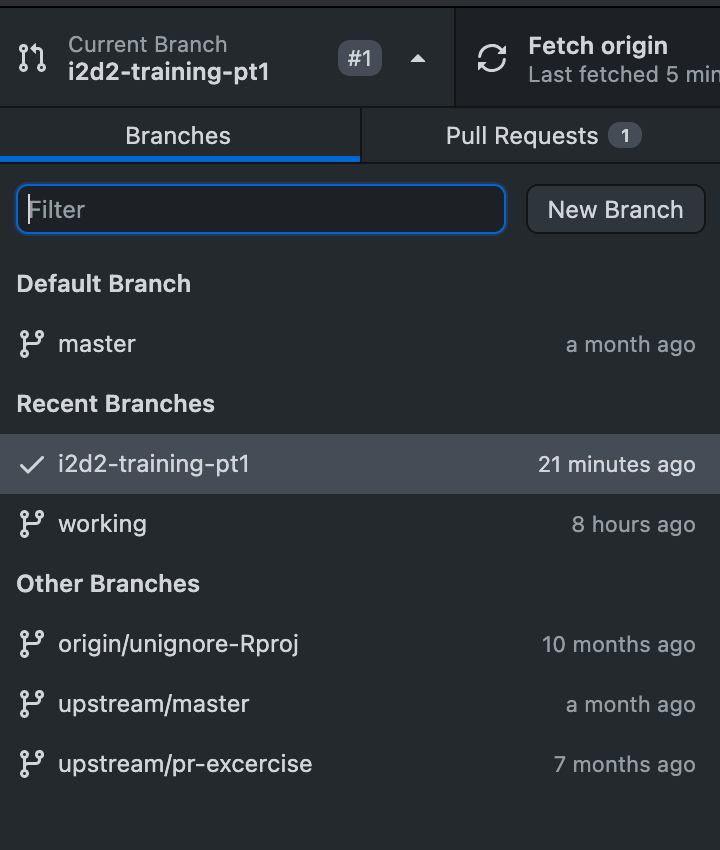
\includegraphics[width=1\linewidth]{img/desktop_branch}

\end{frame}

\begin{frame}
\frametitle{Reclone}

	Everything on the website version of the repo looks good, but I'm getting weird errors locally.

	\begin{itemize}
		\item a. Time for a break.
		\item b. Make a new branch.
		\item c. Just reclone the repo. You can always archive the old local version if you're nervous.
	\end{itemize}

\includegraphics[width=1\linewidth]{img/clonedownload_button}

\end{frame}

\begin{frame}
\frametitle{Just Ask}

	\textbf{When in doubt, just ask someone}

	\vspace{1cm}
	\begin{itemize}
		\item Everybody's learning
		\item Technically, almost anything can be undone, and the earlier the better
		\item Asking directions phenomenon
	\end{itemize}


\end{frame}

\section{Next steps for the research team}

\begin{frame}
\frametitle{Three common GitHub Roles}

	\input{../../Common-Resources/slides/GitHub-Roles.tex}

\end{frame}

\begin{frame}
\frametitle{Next steps for the research team}

	DIME thinks we should do the following:

	\begin{itemize}
		\item Who will be repo maintainer
		\item Agree on a work flow
		\item Public/private repository
		\item External collaborators
		\item Where to put data and where to put code
		\item Request a repo on DIME or World Bank account
	\end{itemize}

\end{frame}

\input{../../Common-Resources/slides/GitHub-Links.tex}

\input{../../Common-Resources/slides/GitHub-Commit-URL.tex}


\end{document}
